% ===========================================================================
%  TikuOS — Memory Management: Arena Allocator
%  Beamer Presentation
% ===========================================================================
\documentclass[aspectratio=169, 10pt]{beamer}

% ---- Theme ----------------------------------------------------------------
\usetheme{Madrid}
\usecolortheme{whale}
\setbeamertemplate{navigation symbols}{}
\setbeamertemplate{footline}{%
  \leavevmode\hbox{%
    \begin{beamercolorbox}[wd=.33\paperwidth,ht=2.5ex,dp=1ex,center]{author in head/foot}%
      \usebeamerfont{author in head/foot}\insertshortauthor
    \end{beamercolorbox}%
    \begin{beamercolorbox}[wd=.34\paperwidth,ht=2.5ex,dp=1ex,center]{title in head/foot}%
      \usebeamerfont{title in head/foot}\insertshorttitle
    \end{beamercolorbox}%
    \begin{beamercolorbox}[wd=.33\paperwidth,ht=2.5ex,dp=1ex,right]{date in head/foot}%
      \usebeamerfont{date in head/foot}\insertshortdate{}\hspace*{2em}%
      \insertframenumber{}/\inserttotalframenumber\hspace*{2ex}
    \end{beamercolorbox}}%
  \vskip0pt%
}

% ---- Packages -------------------------------------------------------------
\usepackage{listings}
\usepackage{graphicx}
\usepackage{hyperref}
\usepackage{booktabs}
\usepackage{multirow}
\usepackage{tikz}
\usetikzlibrary{arrows.meta, positioning, shapes.geometric, calc, decorations.pathreplacing}

% ---- Code listing style ---------------------------------------------------
\lstset{
  basicstyle=\ttfamily\scriptsize,
  keywordstyle=\color{blue}\bfseries,
  commentstyle=\color{gray},
  stringstyle=\color{red!70!black},
  showstringspaces=false,
  breaklines=true,
  frame=single,
  rulecolor=\color{black!30},
  backgroundcolor=\color{blue!3},
  tabsize=4,
}
\lstdefinestyle{cstyle}{
  language=C,
  morekeywords={uint8_t,uint16_t,uint32_t,tiku_arena_t,tiku_mem_stats_t,
                tiku_mem_err_t,tiku_mem_arch_size_t,TIKU_MEM_OK,
                TIKU_MEM_ERR_INVALID,TIKU_MEM_ERR_NOMEM,NULL},
}
\lstdefinestyle{bashstyle}{
  language=bash,
  morekeywords={sudo,apt,make,gcc},
}

% ---- Metadata -------------------------------------------------------------
\title[TikuOS Memory]{TikuOS Memory Management}
\subtitle{Simple. Ubiquitous. Intelligence, Everywhere.}
\author[Ambuj Varshney]{Ambuj Varshney \\ \texttt{ambuj@tiku-os.org}}
\date{\today}

% ===========================================================================
\begin{document}

% ---------------------------------------------------------------------------
\begin{frame}
\titlepage
\end{frame}

% ---------------------------------------------------------------------------
\begin{frame}{Outline}
\tableofcontents
\end{frame}

% ===========================================================================
\section{Why Arena Allocation?}
% ===========================================================================

\begin{frame}{The Problem with malloc/free on MCUs}
\begin{columns}[T]
\begin{column}{0.48\textwidth}
\textbf{Traditional heap (malloc/free):}
\begin{itemize}
  \item Per-object metadata overhead
  \item External fragmentation over time
  \item No MMU to reclaim fragments
  \item Non-deterministic allocation time
  \item Fatal on 2--8\,KB SRAM
\end{itemize}

\vspace{0.5em}
\begin{alertblock}{Fragmentation is Fatal}
On an MCU with 2\,KB SRAM and no MMU, a fragmented heap can make
50\% of memory permanently unusable.
\end{alertblock}
\end{column}

\begin{column}{0.48\textwidth}
\textbf{Arena (bump-pointer) allocator:}
\begin{itemize}
  \item O(1) allocation --- advance a pointer
  \item Zero per-object metadata
  \item Zero fragmentation
  \item Bulk free by resetting the pointer
  \item Deterministic timing
\end{itemize}

\vspace{0.5em}
\begin{block}{Ideal Use Cases}
Temporary buffers, packet processing, sensor data batching ---
any scenario where allocations share a common lifetime.
\end{block}
\end{column}
\end{columns}
\end{frame}

% ===========================================================================
\section{Architecture \& Data Structures}
% ===========================================================================

\begin{frame}[fragile]{Arena Control Block}
\begin{columns}[T]
\begin{column}{0.50\textwidth}
\begin{lstlisting}[style=cstyle, title={kernel/memory/tiku\_mem.h}]
typedef struct {
    uint8_t *buf;
    tiku_mem_arch_size_t capacity;
    tiku_mem_arch_size_t offset;
    tiku_mem_arch_size_t peak;
    tiku_mem_arch_size_t count;
    uint8_t id;
    uint8_t active;
} tiku_arena_t;
\end{lstlisting}
\end{column}

\begin{column}{0.46\textwidth}
\begin{tabular}{@{}lp{4.5cm}@{}}
\toprule
\textbf{Field} & \textbf{Purpose} \\
\midrule
\texttt{buf}      & Caller-provided backing buffer \\
\texttt{capacity} & Total buffer size (bytes) \\
\texttt{offset}   & Current bump pointer \\
\texttt{peak}     & Lifetime high-water mark \\
\texttt{count}    & Allocations since last reset \\
\texttt{id}       & Debug identifier (0--255) \\
\texttt{active}   & Non-zero if initialized \\
\bottomrule
\end{tabular}
\end{column}
\end{columns}

\vspace{0.5em}
\begin{block}{Key Design}
The arena \textbf{does not own} the buffer --- the caller provides a
statically allocated array. No dynamic allocation anywhere.
\end{block}
\end{frame}

% ---------------------------------------------------------------------------
\begin{frame}[fragile]{Supporting Types}
\begin{columns}[T]
\begin{column}{0.48\textwidth}
\begin{lstlisting}[style=cstyle, title={Error codes}]
typedef enum {
    TIKU_MEM_OK         =  0,
    TIKU_MEM_ERR_INVALID = -1,
    TIKU_MEM_ERR_NOMEM  = -2
} tiku_mem_err_t;
\end{lstlisting}

\begin{lstlisting}[style=cstyle, title={Statistics snapshot}]
typedef struct {
    tiku_mem_arch_size_t total_bytes;
    tiku_mem_arch_size_t used_bytes;
    tiku_mem_arch_size_t peak_bytes;
    tiku_mem_arch_size_t alloc_count;
} tiku_mem_stats_t;
\end{lstlisting}
\end{column}

\begin{column}{0.48\textwidth}
\begin{lstlisting}[style=cstyle, title={arch/msp430/tiku\_mem\_arch.h}]
/* MSP430: 16-bit arch, SRAM <= 64 KB
   uint16_t saves RAM vs uint32_t */
typedef uint16_t
    tiku_mem_arch_size_t;

/* 2-byte alignment: unaligned word
   access causes bus fault */
#define TIKU_MEM_ARCH_ALIGNMENT 2U
\end{lstlisting}

\vspace{0.5em}
\begin{block}{Portability}
Change \texttt{ALIGNMENT} and size type to port to 32/64-bit targets.
\end{block}
\end{column}
\end{columns}
\end{frame}

% ---------------------------------------------------------------------------
\begin{frame}[fragile]{How the Bump Pointer Works}
\begin{center}
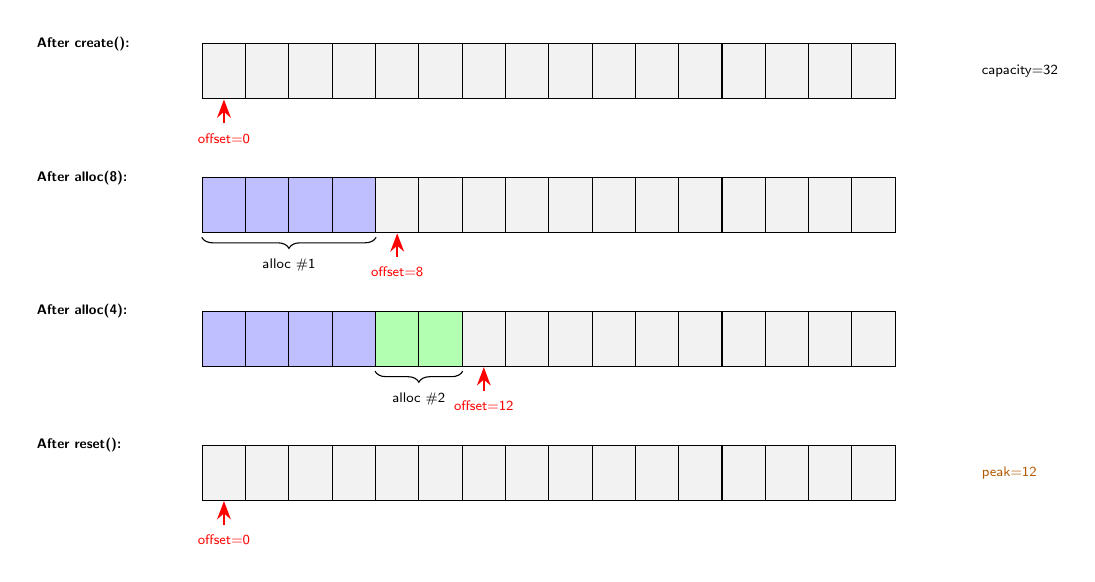
\begin{tikzpicture}[
    cell/.style={draw, minimum width=0.55cm, minimum height=0.7cm, font=\tiny\ttfamily},
    label/.style={font=\tiny\sffamily},
    >=Stealth
  ]

  % --- State 1: After create ---
  \node[label, anchor=west] at (-2.5, 0.35) {\textbf{After create():}};
  \foreach \i in {0,...,15} {
    \node[cell, fill=gray!10] (a\i) at (\i*0.55, 0) {};
  }
  \draw[thick, red, ->] ([yshift=-0.3cm]a0.south) -- (a0.south)
    node[below=0.3cm, font=\tiny\sffamily, red] {offset=0};
  \node[label, anchor=west] at (9.5, 0) {capacity=32};

  % --- State 2: After alloc(8) ---
  \node[label, anchor=west] at (-2.5, -1.35) {\textbf{After alloc(8):}};
  \foreach \i in {0,...,3} {
    \node[cell, fill=blue!25] (b\i) at (\i*0.55, -1.7) {};
  }
  \foreach \i in {4,...,15} {
    \node[cell, fill=gray!10] (b\i) at (\i*0.55, -1.7) {};
  }
  \draw[thick, red, ->] ([yshift=-0.3cm]b4.south) -- (b4.south)
    node[below=0.3cm, font=\tiny\sffamily, red] {offset=8};
  \draw[decorate, decoration={brace, amplitude=4pt, mirror}]
    ([yshift=-0.05cm]b0.south west) -- ([yshift=-0.05cm]b3.south east)
    node[midway, below=0.15cm, font=\tiny\sffamily] {alloc \#1};

  % --- State 3: After alloc(4) ---
  \node[label, anchor=west] at (-2.5, -3.05) {\textbf{After alloc(4):}};
  \foreach \i in {0,...,3} {
    \node[cell, fill=blue!25] (c\i) at (\i*0.55, -3.4) {};
  }
  \foreach \i in {4,...,5} {
    \node[cell, fill=green!30] (c\i) at (\i*0.55, -3.4) {};
  }
  \foreach \i in {6,...,15} {
    \node[cell, fill=gray!10] (c\i) at (\i*0.55, -3.4) {};
  }
  \draw[thick, red, ->] ([yshift=-0.3cm]c6.south) -- (c6.south)
    node[below=0.3cm, font=\tiny\sffamily, red] {offset=12};
  \draw[decorate, decoration={brace, amplitude=4pt, mirror}]
    ([yshift=-0.05cm]c4.south west) -- ([yshift=-0.05cm]c5.south east)
    node[midway, below=0.15cm, font=\tiny\sffamily] {alloc \#2};

  % --- State 4: After reset() ---
  \node[label, anchor=west] at (-2.5, -4.75) {\textbf{After reset():}};
  \foreach \i in {0,...,15} {
    \node[cell, fill=gray!10] (d\i) at (\i*0.55, -5.1) {};
  }
  \draw[thick, red, ->] ([yshift=-0.3cm]d0.south) -- (d0.south)
    node[below=0.3cm, font=\tiny\sffamily, red] {offset=0};
  \node[label, anchor=west, orange!70!black] at (9.5, -5.1) {peak=12};

\end{tikzpicture}
\end{center}
\end{frame}

% ===========================================================================
\section{API Reference}
% ===========================================================================

\begin{frame}[fragile]{tiku\_arena\_create()}
\begin{lstlisting}[style=cstyle]
tiku_mem_err_t tiku_arena_create(tiku_arena_t *arena,
                                 uint8_t *buf,
                                 tiku_mem_arch_size_t size,
                                 uint8_t id);
\end{lstlisting}

\begin{itemize}
  \item Initializes an arena over a \textbf{caller-provided} static buffer
  \item Sets offset, peak, count to 0; marks arena as active
  \item Returns \texttt{TIKU\_MEM\_ERR\_INVALID} if \texttt{arena} or \texttt{buf} is NULL
\end{itemize}

\vspace{0.3em}
\textbf{Usage:}
\begin{lstlisting}[style=cstyle]
static uint8_t buffer[256];
static tiku_arena_t arena;

tiku_mem_err_t err = tiku_arena_create(&arena, buffer, sizeof(buffer), 1);
if (err != TIKU_MEM_OK) {
    /* handle error */
}
\end{lstlisting}
\end{frame}

% ---------------------------------------------------------------------------
\begin{frame}[fragile]{tiku\_arena\_alloc()}
\begin{lstlisting}[style=cstyle]
void *tiku_arena_alloc(tiku_arena_t *arena, tiku_mem_arch_size_t size);
\end{lstlisting}

\begin{itemize}
  \item Bump-pointer allocation --- \textbf{O(1)} complexity
  \item Automatically aligns to \texttt{TIKU\_MEM\_ARCH\_ALIGNMENT} (2 bytes on MSP430)
  \item Updates peak (high-water mark) and allocation count
  \item Returns \texttt{NULL} if: arena is NULL/inactive, size is 0, or arena is full
\end{itemize}

\vspace{0.3em}
\textbf{Usage:}
\begin{lstlisting}[style=cstyle]
/* Allocate a sensor reading buffer */
uint16_t *readings = tiku_arena_alloc(&arena, 10 * sizeof(uint16_t));
if (readings == NULL) {
    /* arena full */
}

/* Odd sizes are rounded up: alloc(3) uses 4 bytes (2-byte alignment) */
uint8_t *pkt = tiku_arena_alloc(&arena, 3);  /* actually uses 4 bytes */
\end{lstlisting}
\end{frame}

% ---------------------------------------------------------------------------
\begin{frame}[fragile]{Alignment: align\_up()}
\begin{lstlisting}[style=cstyle, title={kernel/memory/tiku\_mem.c (private helper)}]
static tiku_mem_arch_size_t align_up(tiku_mem_arch_size_t size)
{
    const tiku_mem_arch_size_t mask = TIKU_MEM_ARCH_ALIGNMENT - 1U;
    return (size + mask) & ~mask;
}
/* Example (alignment = 2): 1 -> 2, 2 -> 2, 3 -> 4, 5 -> 6 */
/* Example (alignment = 4): 1 -> 4, 3 -> 4, 5 -> 8, 8 -> 8 */
\end{lstlisting}

\vspace{0.3em}
\begin{block}{Why Alignment Matters}
\begin{itemize}
  \item MSP430 is a 16-bit architecture --- unaligned word access causes a \textbf{bus fault}
  \item Every returned pointer must be on an even address boundary
  \item The formula \texttt{(size + (align-1)) \& \textasciitilde(align-1)} rounds up to the next multiple
  \item Platform-independent: change \texttt{TIKU\_MEM\_ARCH\_ALIGNMENT} for 32/64-bit
\end{itemize}
\end{block}
\end{frame}

% ---------------------------------------------------------------------------
\begin{frame}[fragile]{tiku\_arena\_reset() vs tiku\_arena\_secure\_reset()}
\begin{columns}[T]
\begin{column}{0.48\textwidth}
\begin{lstlisting}[style=cstyle, title={Normal reset --- O(1)}]
tiku_mem_err_t
tiku_arena_reset(tiku_arena_t *arena)
{
    if (arena == NULL)
        return TIKU_MEM_ERR_INVALID;

    arena->offset = 0;
    arena->count  = 0;
    /* peak preserved */

    return TIKU_MEM_OK;
}
\end{lstlisting}

\begin{itemize}
  \item \textbf{Does NOT zero memory}
  \item \textasciitilde6 cycles regardless of buffer size
  \item Use for general-purpose reuse
\end{itemize}
\end{column}

\begin{column}{0.48\textwidth}
\begin{lstlisting}[style=cstyle, title={Secure reset --- O(n)}]
tiku_mem_err_t
tiku_arena_secure_reset(
    tiku_arena_t *arena)
{
    if (arena == NULL)
        return TIKU_MEM_ERR_INVALID;

    tiku_mem_arch_secure_wipe(
        arena->buf, arena->capacity);

    arena->offset = 0;
    arena->count  = 0;

    return TIKU_MEM_OK;
}
\end{lstlisting}

\begin{itemize}
  \item \textbf{Zeros entire buffer}
  \item \textasciitilde5 cycles/byte on MSP430
  \item Use for crypto keys, credentials
\end{itemize}
\end{column}
\end{columns}
\end{frame}

% ---------------------------------------------------------------------------
\begin{frame}[fragile]{Secure Wipe: Architecture Layer}
\begin{lstlisting}[style=cstyle, title={arch/msp430/tiku\_mem\_arch.c}]
void tiku_mem_arch_secure_wipe(uint8_t *buf, tiku_mem_arch_size_t len)
{
    volatile uint8_t *p = (volatile uint8_t *)buf;
    tiku_mem_arch_size_t i;

    for (i = 0; i < len; i++) {
        p[i] = 0;
    }
}
\end{lstlisting}

\vspace{0.3em}
\begin{alertblock}{Why \texttt{volatile}?}
Without it, GCC \texttt{-O2} sees the buffer is never read after zeroing and
\textbf{elides the entire loop}. The \texttt{volatile} qualifier forces every
store to execute.
\end{alertblock}

\vspace{0.3em}
\begin{table}
\centering
\small
\begin{tabular}{@{}rrr@{}}
\toprule
\textbf{Buffer Size} & \textbf{Cycles (MSP430X)} & \textbf{Time @ 16\,MHz} \\
\midrule
64\,B   &   \textasciitilde320  & 20\,$\mu$s  \\
256\,B  &  \textasciitilde1280  & 80\,$\mu$s  \\
2048\,B & \textasciitilde10240  & 640\,$\mu$s \\
\bottomrule
\end{tabular}
\end{table}
\end{frame}

% ---------------------------------------------------------------------------
\begin{frame}[fragile]{tiku\_arena\_stats()}
\begin{lstlisting}[style=cstyle]
tiku_mem_err_t tiku_arena_stats(const tiku_arena_t *arena,
                                tiku_mem_stats_t *stats);
\end{lstlisting}

\begin{itemize}
  \item Returns a snapshot: total, used, peak, and allocation count
  \item O(1) --- direct field copy
  \item Returns \texttt{TIKU\_MEM\_ERR\_INVALID} if either pointer is NULL
\end{itemize}

\vspace{0.3em}
\textbf{Usage:}
\begin{lstlisting}[style=cstyle]
tiku_mem_stats_t stats;

tiku_arena_stats(&arena, &stats);

TIKU_PRINTF("Total: %u B\n", stats.total_bytes);
TIKU_PRINTF("Used:  %u B\n", stats.used_bytes);
TIKU_PRINTF("Peak:  %u B\n", stats.peak_bytes);   /* lifetime max */
TIKU_PRINTF("Count: %u\n",   stats.alloc_count);
\end{lstlisting}

\vspace{0.3em}
\begin{block}{Peak Tracking}
\texttt{peak\_bytes} records the lifetime high-water mark ---
it \textbf{never decreases}, even across resets.
Useful for capacity planning and right-sizing buffers.
\end{block}
\end{frame}

% ===========================================================================
\section{Complete Usage Example}
% ===========================================================================

\begin{frame}[fragile]{End-to-End Example}
\begin{lstlisting}[style=cstyle]
/* 1. Declare a static buffer and arena */
static uint8_t sensor_buf[128];
static tiku_arena_t sensor_arena;

void process_sensor_data(void) {
    tiku_mem_stats_t stats;

    /* 2. Create the arena once */
    tiku_arena_create(&sensor_arena, sensor_buf, sizeof(sensor_buf), 1);

    /* 3. Allocate temporary buffers */
    uint16_t *raw = tiku_arena_alloc(&sensor_arena, 10 * sizeof(uint16_t));
    uint8_t  *pkt = tiku_arena_alloc(&sensor_arena, 24);

    if (raw == NULL || pkt == NULL) {
        /* arena full - handle gracefully */
        return;
    }

    /* 4. Use the memory ... */
    read_sensors(raw, 10);
    format_packet(pkt, raw, 10);
    transmit(pkt, 24);

    /* 5. Check stats, then reset for next cycle */
    tiku_arena_stats(&sensor_arena, &stats);
    /* stats.peak_bytes tells you the max ever used */

    tiku_arena_reset(&sensor_arena);  /* O(1) - ready for reuse */
}
\end{lstlisting}
\end{frame}

% ---------------------------------------------------------------------------
\begin{frame}[fragile]{Multi-Arena Pattern}
\begin{lstlisting}[style=cstyle]
/* Two independent arenas for different subsystems */
static uint8_t net_buf[64];
static uint8_t crypto_buf[32];
static tiku_arena_t net_arena, crypto_arena;

void init(void) {
    tiku_arena_create(&net_arena,    net_buf,    sizeof(net_buf),    10);
    tiku_arena_create(&crypto_arena, crypto_buf, sizeof(crypto_buf), 20);
}

void on_packet_received(void) {
    uint8_t *frame = tiku_arena_alloc(&net_arena, 48);
    /* ... process frame ... */
    tiku_arena_reset(&net_arena);             /* O(1) reuse */
}

void on_auth_complete(void) {
    uint8_t *key = tiku_arena_alloc(&crypto_arena, 16);
    /* ... use key ... */
    tiku_arena_secure_reset(&crypto_arena);   /* wipe secrets */
}
\end{lstlisting}

\begin{block}{Independence}
Each arena has its own buffer, offset, peak, and count.
Resetting one does not affect the other.
\end{block}
\end{frame}

% ===========================================================================
\section{File Organization}
% ===========================================================================

\begin{frame}[fragile]{Memory Module Files}
\begin{table}
\centering
\small
\begin{tabular}{@{}lll@{}}
\toprule
\textbf{Layer} & \textbf{File} & \textbf{Role} \\
\midrule
\multirow{2}{*}{Kernel (portable)}
  & \texttt{kernel/memory/tiku\_mem.h} & Public API, types, docs \\
  & \texttt{kernel/memory/tiku\_mem.c} & Arena logic, \texttt{align\_up()} \\
\midrule
\multirow{2}{*}{Arch (MSP430)}
  & \texttt{arch/msp430/tiku\_mem\_arch.h} & Alignment, size type \\
  & \texttt{arch/msp430/tiku\_mem\_arch.c} & Secure wipe, arch init \\
\midrule
\multirow{2}{*}{Tests}
  & \texttt{tests/test\_tiku\_mem.c} & 9 test cases \\
  & \texttt{tests/tiku\_test\_config.h} & Per-test enable flags \\
\bottomrule
\end{tabular}
\end{table}

\vspace{0.5em}
\begin{block}{Porting to a New Architecture}
Only two files need to change:
\begin{enumerate}
  \item Set \texttt{TIKU\_MEM\_ARCH\_ALIGNMENT} (e.g., 4 for ARM Cortex-M)
  \item Set \texttt{tiku\_mem\_arch\_size\_t} (e.g., \texttt{uint32\_t} for 32-bit)
  \item Implement \texttt{tiku\_mem\_arch\_secure\_wipe()} if needed
\end{enumerate}
\end{block}
\end{frame}

% ===========================================================================
\section{API Summary}
% ===========================================================================

\begin{frame}{API at a Glance}
\begin{table}
\centering
\small
\begin{tabular}{@{}llll@{}}
\toprule
\textbf{Function} & \textbf{Returns} & \textbf{Complexity} & \textbf{Description} \\
\midrule
\texttt{tiku\_arena\_create}  & \texttt{err\_t} & O(1) & Init arena over static buffer \\
\texttt{tiku\_arena\_alloc}   & \texttt{void*}  & O(1) & Bump-pointer allocation \\
\texttt{tiku\_arena\_reset}   & \texttt{err\_t} & O(1) & Reset offset; preserve peak \\
\texttt{tiku\_arena\_secure\_reset} & \texttt{err\_t} & O(n) & Zero buffer + reset \\
\texttt{tiku\_arena\_stats}   & \texttt{err\_t} & O(1) & Snapshot of arena state \\
\texttt{tiku\_mem\_init}      & \texttt{void}   & O(1) & Module initialization \\
\bottomrule
\end{tabular}
\end{table}

\vspace{0.5em}
\begin{columns}[T]
\begin{column}{0.48\textwidth}
\begin{block}{Error Handling}
\begin{itemize}
  \item NULL checks on every public function
  \item \texttt{alloc()} returns NULL on failure
  \item Others return \texttt{tiku\_mem\_err\_t}
  \item No assertions --- safe for production
\end{itemize}
\end{block}
\end{column}
\begin{column}{0.48\textwidth}
\begin{block}{Design Guarantees}
\begin{itemize}
  \item No dynamic allocation anywhere
  \item No individual free (by design)
  \item All pointers naturally aligned
  \item Peak survives all resets
\end{itemize}
\end{block}
\end{column}
\end{columns}
\end{frame}

% ===========================================================================
\section{Test Suite}
% ===========================================================================

\begin{frame}[fragile]{Test Configuration}
\begin{columns}[T]
\begin{column}{0.48\textwidth}
\begin{lstlisting}[style=cstyle, title={tests/tiku\_test\_config.h}]
/* Master enable */
#define TEST_ENABLE 1

/* Memory test flags */
#define TEST_MEM_CREATE       1
#define TEST_MEM_ALLOC        1
#define TEST_MEM_ALIGNMENT    1
#define TEST_MEM_FULL         1
#define TEST_MEM_RESET        1
#define TEST_MEM_PEAK         1
#define TEST_MEM_INVALID      1
#define TEST_MEM_SECURE_RESET 1
#define TEST_MEM_TWO_ARENAS   1
\end{lstlisting}
\end{column}

\begin{column}{0.48\textwidth}
\textbf{On-target:}
\begin{lstlisting}[style=bashstyle]
# Enable flags in tiku_test_config.h
# then build and flash
make flash MCU=msp430fr5969
make monitor
\end{lstlisting}

\vspace{0.5em}
\textbf{Host-native (no hardware):}
\begin{lstlisting}[style=bashstyle]
gcc -std=c99 -Wall -Wextra -I. \
  tests/test_tiku_mem.c \
  kernel/memory/tiku_mem.c \
  -o test_tiku_mem \
  && ./test_tiku_mem
\end{lstlisting}

\vspace{0.3em}
Host mode provides portable stubs for arch functions ---
no MSP430 toolchain required.
\end{column}
\end{columns}
\end{frame}

% ---------------------------------------------------------------------------
\begin{frame}{Test Cases Overview}
\begin{table}
\centering
\small
\begin{tabular}{@{}clp{7cm}@{}}
\toprule
\textbf{\#} & \textbf{Test Flag} & \textbf{What It Verifies} \\
\midrule
1 & \texttt{TEST\_MEM\_CREATE}    & Arena becomes active; ID set; initial stats zero \\
2 & \texttt{TEST\_MEM\_ALLOC}     & Non-NULL pointers; sequential placement; non-overlap \\
3 & \texttt{TEST\_MEM\_ALIGNMENT} & Odd requests rounded up; all pointers aligned \\
4 & \texttt{TEST\_MEM\_FULL}      & NULL returned when arena exhausted; boundary check \\
5 & \texttt{TEST\_MEM\_RESET}     & Offset/count reset to 0; peak preserved; reallocation works \\
6 & \texttt{TEST\_MEM\_PEAK}      & Peak increases; never decreases; survives resets \\
7 & \texttt{TEST\_MEM\_INVALID}   & NULL arena/buf rejected; zero-size returns NULL \\
8 & \texttt{TEST\_MEM\_SECURE\_RESET} & Buffer zeroed; state reset; peak preserved \\
9 & \texttt{TEST\_MEM\_TWO\_ARENAS}   & Independent arenas; separate stats; reset isolation \\
\bottomrule
\end{tabular}
\end{table}
\end{frame}

% ---------------------------------------------------------------------------
\begin{frame}[fragile]{Test Deep Dive: Allocation \& Alignment}
\begin{lstlisting}[style=cstyle, title={test\_tiku\_mem.c --- Allocation test}]
uint8_t buf[64];
tiku_arena_t arena;
tiku_arena_create(&arena, buf, sizeof(buf), 1);

/* Allocate 8 bytes */
void *p1 = tiku_arena_alloc(&arena, 8);
TEST_ASSERT(p1 != NULL);
TEST_ASSERT(p1 == buf);                 /* starts at base */

/* Second allocation is sequential */
void *p2 = tiku_arena_alloc(&arena, 4);
TEST_ASSERT(p2 == buf + 8);             /* right after p1 */
TEST_ASSERT((uintptr_t)p2 % TIKU_MEM_ARCH_ALIGNMENT == 0);
\end{lstlisting}

\begin{lstlisting}[style=cstyle, title={test\_tiku\_mem.c --- Alignment test}]
/* Odd request: 3 bytes -> rounded to 4 (alignment=2) */
void *p1 = tiku_arena_alloc(&arena, 3);
void *p2 = tiku_arena_alloc(&arena, 1);

/* p2 starts at offset 4, not 3 */
TEST_ASSERT((uint8_t *)p2 - (uint8_t *)p1 >= 4);
TEST_ASSERT((uintptr_t)p2 % TIKU_MEM_ARCH_ALIGNMENT == 0);
\end{lstlisting}
\end{frame}

% ---------------------------------------------------------------------------
\begin{frame}[fragile]{Test Deep Dive: Peak Tracking \& Secure Reset}
\begin{lstlisting}[style=cstyle, title={test\_tiku\_mem.c --- Peak tracking across resets}]
tiku_mem_stats_t stats;

/* Cycle 1: allocate 12 bytes */
tiku_arena_alloc(&arena, 12);
tiku_arena_stats(&arena, &stats);
TEST_ASSERT(stats.peak_bytes == 12);

tiku_arena_reset(&arena);

/* Cycle 2: allocate 32 bytes -> peak grows */
tiku_arena_alloc(&arena, 32);
tiku_arena_stats(&arena, &stats);
TEST_ASSERT(stats.peak_bytes == 32);

tiku_arena_reset(&arena);

/* Cycle 3: allocate only 8 -> peak stays at 32 */
tiku_arena_alloc(&arena, 8);
tiku_arena_stats(&arena, &stats);
TEST_ASSERT(stats.peak_bytes == 32);   /* never decreases */
\end{lstlisting}

\begin{lstlisting}[style=cstyle, title={test\_tiku\_mem.c --- Secure reset}]
/* Fill with 0xAA, then secure reset */
memset(buf, 0xAA, sizeof(buf));
tiku_arena_secure_reset(&arena);
for (i = 0; i < sizeof(buf); i++)
    TEST_ASSERT(buf[i] == 0x00);       /* every byte wiped */
\end{lstlisting}
\end{frame}

% ---------------------------------------------------------------------------
\begin{frame}[fragile]{Test Deep Dive: Arena Full \& Two Arenas}
\begin{columns}[T]
\begin{column}{0.48\textwidth}
\begin{lstlisting}[style=cstyle, title={Arena full test}]
/* Tiny arena: 4 * alignment bytes */
uint8_t buf[4 * TIKU_MEM_ARCH_ALIGNMENT];
tiku_arena_t arena;
tiku_arena_create(&arena, buf,
    sizeof(buf), 1);

/* First alloc succeeds */
void *p = tiku_arena_alloc(&arena,
    2 * TIKU_MEM_ARCH_ALIGNMENT);
TEST_ASSERT(p != NULL);

/* Fill the rest */
p = tiku_arena_alloc(&arena,
    2 * TIKU_MEM_ARCH_ALIGNMENT);
TEST_ASSERT(p != NULL);

/* Arena exhausted -> NULL */
p = tiku_arena_alloc(&arena, 1);
TEST_ASSERT(p == NULL);
\end{lstlisting}
\end{column}

\begin{column}{0.48\textwidth}
\begin{lstlisting}[style=cstyle, title={Two independent arenas}]
uint8_t buf_a[32], buf_b[64];
tiku_arena_t arena_a, arena_b;

tiku_arena_create(&arena_a,
    buf_a, 32, 10);
tiku_arena_create(&arena_b,
    buf_b, 64, 20);

/* Allocate from both */
tiku_arena_alloc(&arena_a, 16);
tiku_arena_alloc(&arena_b, 32);

/* Reset A only */
tiku_arena_reset(&arena_a);

/* B is unaffected */
tiku_mem_stats_t s;
tiku_arena_stats(&arena_b, &s);
TEST_ASSERT(s.used_bytes == 32);
\end{lstlisting}
\end{column}
\end{columns}
\end{frame}

% ===========================================================================
\section{Summary}
% ===========================================================================

\begin{frame}{Summary}
\begin{columns}[T]
\begin{column}{0.48\textwidth}
\begin{block}{Memory Management Design}
\begin{itemize}
  \item Arena (bump-pointer) allocator
  \item O(1) alloc, O(1) reset
  \item Zero fragmentation
  \item Zero per-object metadata
  \item Static buffers only
  \item Platform-aware alignment
  \item Lifetime peak tracking
  \item Secure wipe for secrets
\end{itemize}
\end{block}
\end{column}

\begin{column}{0.48\textwidth}
\begin{block}{Test Coverage}
\begin{itemize}
  \item 9 comprehensive test cases
  \item Runs on-target or host-native
  \item Per-test enable flags
  \item Covers: create, alloc, alignment, full, reset, peak, invalid inputs, secure reset, multi-arena
\end{itemize}
\end{block}

\vspace{0.3em}
\begin{alertblock}{FRAM Awareness}
Secure reset protects against non-volatile FRAM persistence ---
secrets don't survive across reboots.
\end{alertblock}
\end{column}
\end{columns}
\end{frame}

% ---------------------------------------------------------------------------
\begin{frame}{Thank You}
\begin{center}
\Large\textbf{TikuOS Memory Management}\\[0.5em]
\normalsize Arena Allocator for Physical AI Endpoints\\[1.5em]

\begin{tabular}{rl}
  Repository: & \url{https://github.com/tikuos/tikuOS} \\
  License:    & Apache 2.0 \\
  API Header: & \texttt{kernel/memory/tiku\_mem.h} \\
  Tests:      & \texttt{tests/test\_tiku\_mem.c} \\
\end{tabular}
\end{center}
\end{frame}

\end{document}
